% Figure 1: one sweep of the clock hand. Build with:
%   pdflatex clock_buffer_manager.tex
%   pdftocairo -png -r 200 -singlefile clock_buffer_manager.pdf clock_buffer_manager
\documentclass[tikz,border=8pt]{standalone}
\usepackage[T1]{fontenc}
\usepackage{lmodern}
\usetikzlibrary{arrows.meta}

\definecolor{pinned}{HTML}{BDBDBD}
\definecolor{refset}{HTML}{FFD54F}
\definecolor{victim}{HTML}{EF5350}
\definecolor{last}{HTML}{90CAF9}

\begin{document}
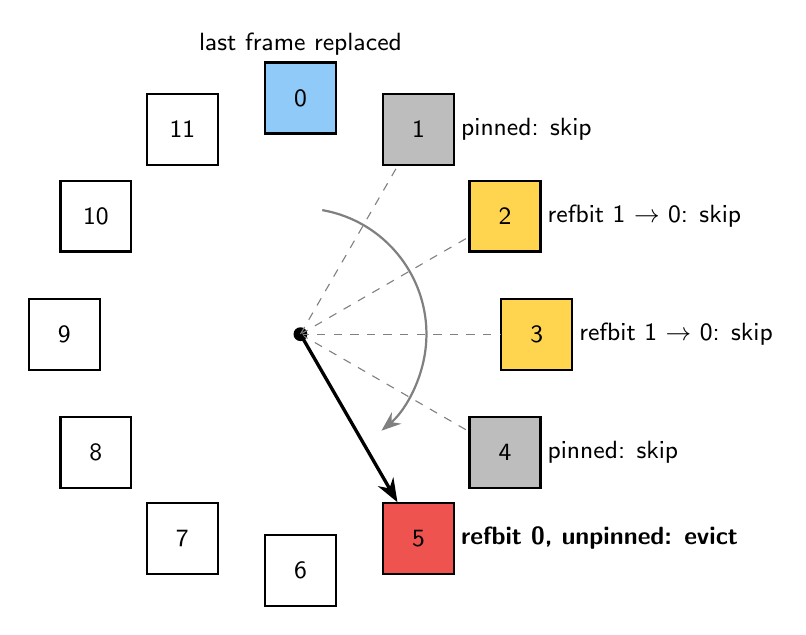
\begin{tikzpicture}[
    font=\sffamily\small,
    frame/.style={draw, thick, minimum size=9mm, inner sep=0pt, fill=white},
    note/.style={inner sep=2pt, align=left},
  ]
  \def\n{12}
  \def\r{3cm}

  % Frames, numbered clockwise from the top. Frame i sits at angle 90 - 30i.
  \foreach \i/\fill in {0/last, 1/pinned, 2/refset, 3/refset, 4/pinned, 5/victim,
                        6/white, 7/white, 8/white, 9/white, 10/white, 11/white} {
    \node[frame, fill=\fill] (f\i) at ({90 - 360/\n*\i}:\r) {\i};
  }

  % Hand: dashed lines to the frames it passes, solid arrow to the victim.
  \fill (0,0) circle (2.5pt);
  \foreach \i in {1,...,4} \draw[dashed, gray] (0,0) -- (f\i);
  \draw[very thick, -{Stealth[length=3mm]}] (0,0) -- (f5);

  % Direction of the sweep.
  \draw[-{Stealth[length=2.5mm]}, gray, thick]
    (80:1.6cm) arc[start angle=80, end angle=-50, radius=1.6cm];

  % What happens at each frame the hand reaches.
  \node[note, anchor=south] at (f0.north) {last frame replaced};
  \node[note, anchor=west] at (f1.east) {pinned: skip};
  \node[note, anchor=west] at (f2.east) {refbit 1 $\to$ 0: skip};
  \node[note, anchor=west] at (f3.east) {refbit 1 $\to$ 0: skip};
  \node[note, anchor=west] at (f4.east) {pinned: skip};
  \node[note, anchor=west] at (f5.east) {\textbf{refbit 0, unpinned: evict}};
\end{tikzpicture}
\end{document}
